\documentclass{article}


% if you need to pass options to natbib, use, e.g.:
%     \PassOptionsToPackage{numbers, compress}{natbib}
% before loading neurips_2022


% ready for submission
% \usepackage{neurips_2022}


% to compile a preprint version, e.g., for submission to arXiv, add add the
% [preprint] option:
%\usepackage[preprint, nonatbib]{neurips_2023}
\usepackage[preprint, nonatbib]{neurips_2023}

% to compile a camera-ready version, add the [final] option, e.g.:
%     \usepackage[final]{neurips_2022}


% to avoid loading the natbib package, add option nonatbib:
    % \usepackage[nonatbib]{neurips_2022}


\usepackage[utf8]{inputenc} % allow utf-8 input
\usepackage[T1]{fontenc}    % use 8-bit T1 fonts
\usepackage{hyperref}       % hyperlinks
\usepackage{url}            % simple URL typesetting
\usepackage{booktabs}       % professional-quality tables
\usepackage{amsfonts}       % blackboard math symbols
\usepackage{nicefrac}       % compact symbols for 1/2, etc.
\usepackage{microtype}      % microtypography
\usepackage{xcolor}         % colors

\usepackage[
    %backend=biber, 
    natbib=true,
    citestyle=numeric-comp,
    bibstyle=ieee,
    sorting=nty
]{biblatex}
\addbibresource{neurips_2023.bib}

\usepackage{graphicx}
\usepackage{caption}
\usepackage{subcaption}
\usepackage{subcaption}
\usepackage{bm}
\usepackage{amsmath,amssymb}
\usepackage{booktabs}
\usepackage{algorithm}
\usepackage[noend]{algorithmic}
\usepackage{multirow}
\usepackage[flushleft]{threeparttable}

\usepackage{multirow}
\usepackage{makecell}
\usepackage{multirow}
\usepackage{xspace}
%\usepackage{hyperref}
%\usepackage{subfigure}
%\usepackage{bm}
\usepackage{color}
\usepackage{wrapfig}
\usepackage{bbding}
%\usepackage{floatrow}
% \usepackage{tikz}
% \newcommand*{\circled}[1]{\lower.7ex\hbox{\tikz\draw (0pt, 0pt)%
%     circle (.5em) node {\makebox[1em][c]{\tiny #1}};}}


\newcommand{\ie}{\emph{i.e.,}\xspace}
\newcommand{\eg}{\emph{e.g.,}\xspace}
\newcommand{\etal}{\emph{et al.}\xspace}
\def\revise{\textcolor{red}}
%%

\newcommand{\yao}[1]{{\color{cyan} YF: #1}}


%\renewcommand{\algorithmicrequire}{\textbf{Input:}}
%\renewcommand{\algorithmicensure}{\textbf{Init:}}
%\renewcommand{\algorithmiccomment}[1]{\hfill// #1}
%\newenvironment{packed_enumerate}{
%	\begin{enumerate}
%		\setlength{\itemsep}{0pt}
%		\setlength{\parskip}{0pt}
%		\setlength{\parsep}{0pt}
%	}{\end{enumerate}
%}
%\setlength{\textfloatsep}{5pt plus 1.0pt minus 2.0pt}
%\setlength{\abovecaptionskip}{3pt plus 3pt minus 2pt}
%\definecolor{f3green}{RGB}{0,144,81}
%\definecolor{f3brown}{RGB}{148,82,0}
%\newtheorem{scalingrule}{Scaling Rule}
%\newtheorem{theorem}{Theorem}
%\newcommand{\innerproduct}[2]{\langle #1, #2 \rangle}

%\DeclareMathOperator*{\E}{\mathbb{E}}
%\DeclareMathOperator*{\prob}{P}
%\DeclareMathOperator*{\g}{\text{\slshape g}}

%\title{An Empirical Study on Further Scaling Large Language Model under Token-Crisis}

\title{To Repeat or Not To Repeat: \\ Insights from Scaling LLM under Token-Crisis}


% The \author macro works with any number of authors. There are two commands
% used to separate the names and addresses of multiple authors: \And and \AND.
%
% Using \And between authors leaves it to LaTeX to determine where to break the
% lines. Using \AND forces a line break at that point. So, if LaTeX puts 3 of 4
% authors names on the first line, and the last on the second line, try using
% \AND instead of \And before the third author name.
\stepcounter{footnote}

%\author{Anonymous Author(s) \\ 
%Address}


\author{
Fuzhao Xue$^{1}$ \quad
Yao Fu$^2$ \quad
Wangchunshu Zhou$^3$ \quad
Zangwei Zheng$^{1}$ \quad
Yang You$^{1}$\thanks{Correspondence to youy@comp.nus.edu.sg} \\
$^1$National University of Singapore \\
$^2$University of Edinburgh \\
$^3$ETH Zurich \\
%yao.fu@ed.ac.uk\\
%wangchunshu.zhou@inf.ethz.ch
%Shenggui Li$^{1,}$ \quad Fuzhao Xue$^{1}$\thanks{Equal Contribution}  \quad Chaitanya Baranwal$^1$ \quad Yongbin Li$^1$ \quad Yang You$^1$\\
%$^1$Department of Computer Science, National University of Singapore
%\{zangwei, f-xue, zihengq, youy\}@comp.nus.edu.sg \\
%\{zouxuan, pengtai.xu, da.tang, zhen.li1, chenguang.xi, peng.wu, leqi.zou,\\ yijie.zhu, ming.chen, xiangzhuo.ding, youlong.cheng\}@bytedance.com
}

\begin{document}


\maketitle


\begin{abstract}

Recent research has highlighted the importance of dataset size in scaling language models. 
However, large language models (LLMs) are notoriously token-hungry during pre-training, and high-quality text data on the web is likely to be approaching its scaling limit for LLMs.
To further enhance LLMs, a straightforward approach is to repeat the pre-training data for additional epochs. 
In this study, we empirically investigate three key aspects under this approach. First, we explore the consequences of repeating pre-training data, revealing that the model is susceptible to overfitting, leading to multi-epoch degradation. Second, we examine the key factors contributing to multi-epoch degradation, finding that significant factors include dataset size, model parameters, and training objectives, while less influential factors consist of dataset quality and model FLOPs. Finally, we explore whether widely used regularization can alleviate multi-epoch degradation. Most regularization techniques do not yield significant improvements, except for dropout, which demonstrates remarkable effectiveness but requires careful tuning when scaling up the model size. Additionally, we discover that leveraging mixture-of-experts (MoE) enables cost-effective and efficient hyper-parameter tuning for computationally intensive dense LLMs with comparable trainable parameters, potentially impacting efficient LLM development on a broader scale.


%and contribute 11 takeaways about further scaling LLM under token-crisis. Some of these takeaways, \eg using mixture-of-experts to tune hyper-parameters of a more computational-expensive dense LLM in a cheaper and faster way, can also have a broader impact on efficient LLM development.


%To address this token-crisis issue, we plan to investigate following approaches: (1) training LLMs with repeated data; (2) training LLMs with data generated by off-the-shelf LLMs; and (3) implementing adaptive parameter activation and computation allocation. Our goal is to explore these directions and enable the community to create more effective LLMs without data constraints.

\end{abstract}



%%%%%%%%%%%%%%%%%%%%%%%%%%%%%%%%%%%%%%%%%%%%%%%%%%%%%%%%%%%%
\printbibliography

\newpage
\appendix

\section{Rebuttal}

\subsection{Encoder-Decoder vs Decoder-Only}
\begin{figure}[h]
\vspace{-0.4cm}
  \begin{center}
    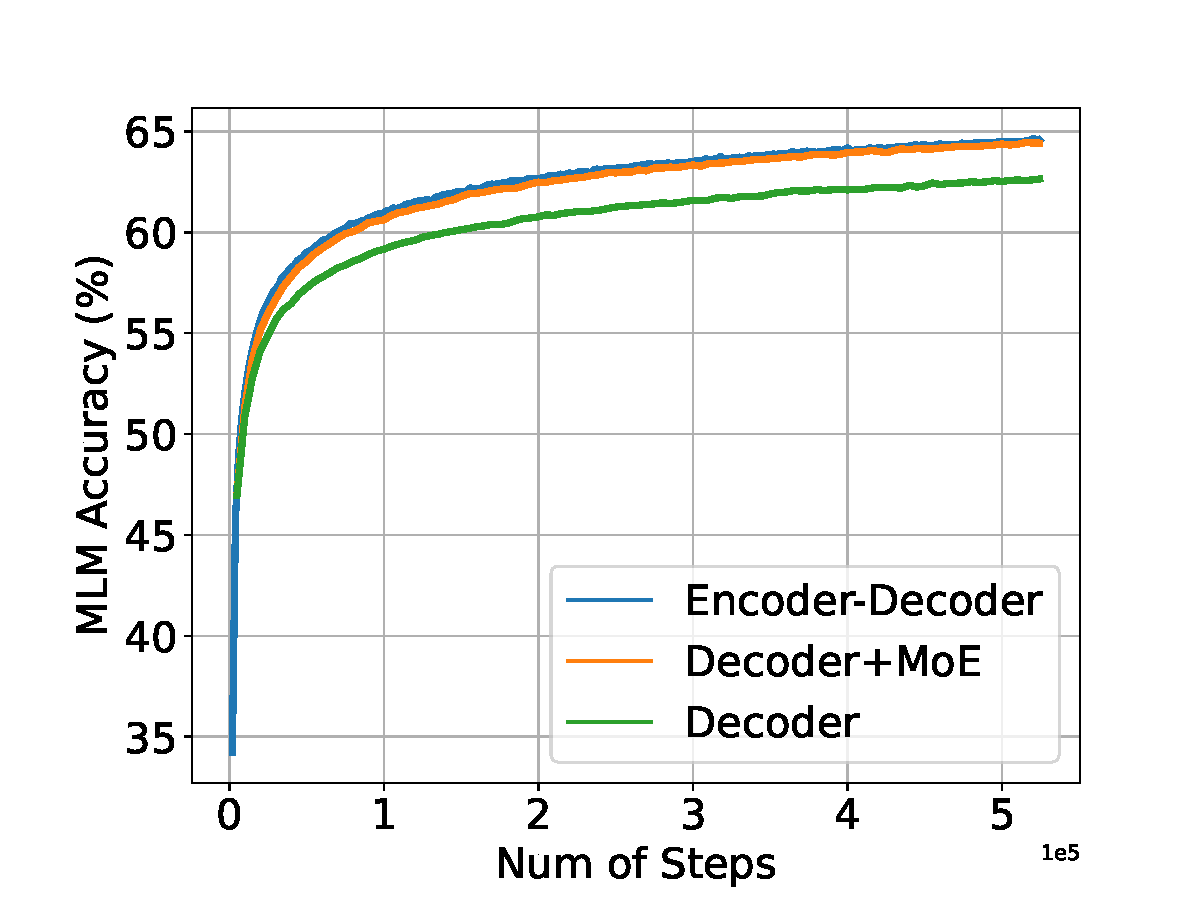
\includegraphics[width=0.4\textwidth]{ende_vs_demoe.pdf}
  \end{center}
  %\vspace{-0.4cm}
  \caption{We train three models (\ie encoder-decoder, decoder-only, MoE-based decoder-only) with the same data and training objective. }\label{fig:ende_de_demoe}
\vspace{-0.3cm}
\end{figure}

We can see encoder-decoder is clearly better than decoder-only but the MoE based decoder-only model having comparable trainable parameters with encoder-decoder performs almost the same as encoder-decoder model.  Therefore, as suggested by UL2 paper, the different behaviours of encoder-decoder and decoder-only are more from the training objective instead of model architecture. That is the reason why we explore UL2 training objective in our Section 3.3.



\subsection{Ablation Study on Batch Size of Larger Dataset Size}\label{sec:ablation-bsz}

\begin{figure}[h]
\vspace{-0.4cm}
  \begin{center}
    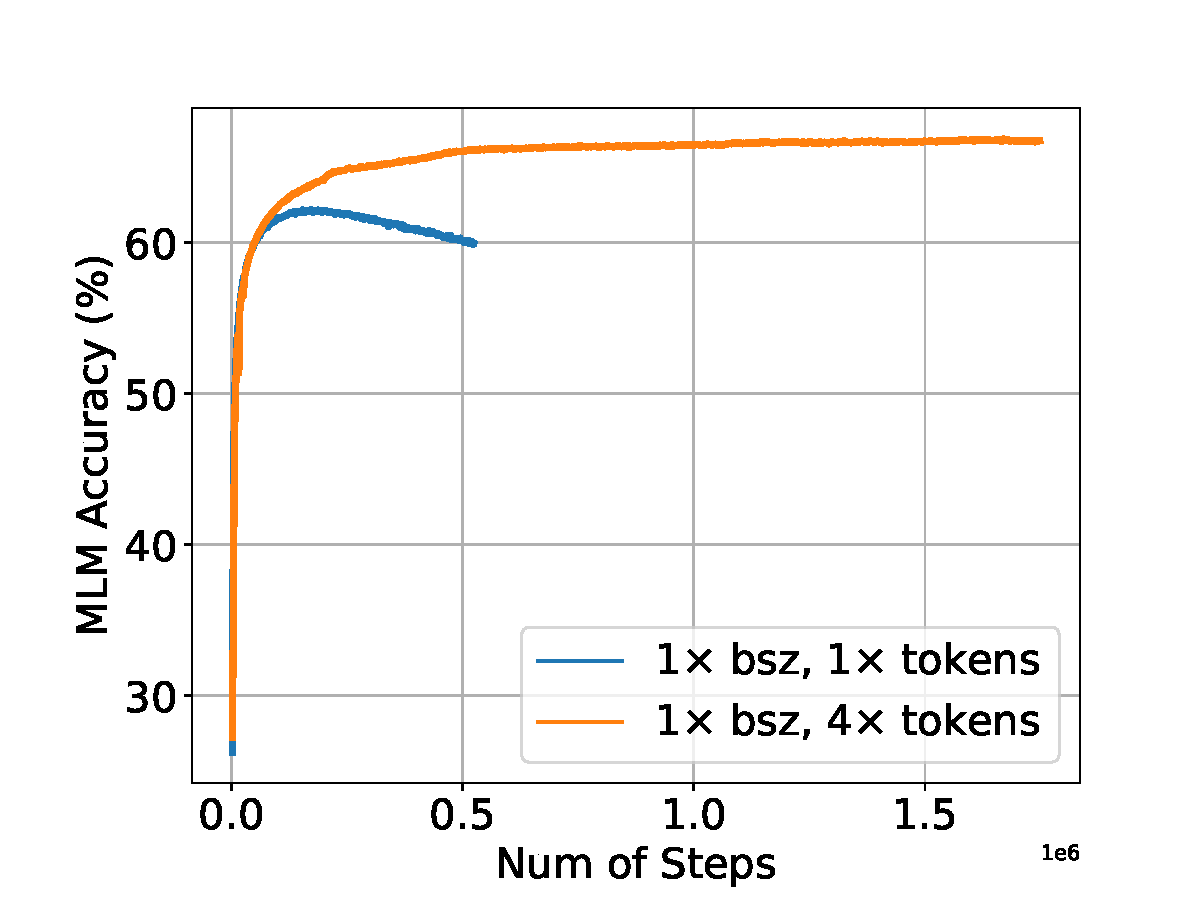
\includegraphics[width=0.4\textwidth]{dataset_size_longer.pdf}
  \end{center}
  %\vspace{-0.4cm}
  \caption{We fix the batch size and number of repeats, and then train the model with 4 times more steps to go through 4 times more tokens.}\label{fig:dataset_size_longer}
\vspace{-0.4cm}
\end{figure}

We can see when using smaller batch size than what we did in Figure~\ref{fig:dataset_size_longer}, model still has little multi-epoch degradation. This further verifies that larger dataset can alleviate the multi-epoch degradation.

\subsection{Downsteam Evaluation}

\begin{table}[h]
\small
\vspace{-0.5cm}
\caption{The updated fine-tuning results. We include the standard deviation of 5 runs.}
\vspace{5pt}
\centering
\begin{tabular}{l ll ll }
\toprule 
Model      & BoolQ  &  RTE      & \multicolumn{2}{l}{SQuAD} \\  \cmidrule(lr){2-2} \cmidrule(lr){3-3} \cmidrule(lr){4-5} 
                & Acc & Acc & EM & F1  \\ \midrule
C4-SpanCorr-Repeat1    & 77.0$\pm$0.7   & 68.9$\pm$0.8     & 82.3$\pm$0.9   & 90.0$\pm$0.9      \\ 
C4-SpanCorr-Repeat$2^{8}$   & 73.8$\pm$1.0   & 66.4$\pm$0.3     & 80.0$\pm$0.6   & 88.1$\pm$0.5      \\ 
C4-UL2-Repeat1       & 78.8$\pm$0.9   & 72.2$\pm$1.2     & 82.3$\pm$0.8   & 90.2$\pm$0.7      \\ 
C4-UL2-Repeat$2^{8}$   & 74.5$\pm$0.6   & 68.4$\pm$0.7     & 79.3$\pm$1.1   & 87.3$\pm$1.2     \\ 
C4-Wiki-Repeat1       & 74.2$\pm$0.7   & 69.3$\pm$1.1     & 82.6$\pm$0.8   & 90.1$\pm$0.6      \\ 
C4-Wiki-Repeat$2^{8}$  & 71.4$\pm$0.4   & 64.9$\pm$0.5     & 79.6$\pm$1.0   & 87.9$\pm$1.3     \\  \bottomrule
\end{tabular}
\label{tbl:downstream}
%\vspace{-0.5cm}
\end{table}


\end{document}